\documentclass{udisc}

% user defs
\usepackage{enumerate} % custom enumeration symbols
\newcommand{\noteCC}[1]{\footnote{{\textbf{CC:} {#1}}}}

% change log
%%%%%%%%%%%%
% - 2024-11-18: added original ISO relation definitions under usage and/or arguments; added ISO notes (CC)
% - 2024-11-18: added notes on corresponding Augsburg relations. these are temporary notes to facilitate comparison/merging, to be omitted from final guidelines (CC)
% - 2024-11-18: replaced @standard in iso.bib by @techreport: didn't compile locally otherwise

% tech issues
%%%%%%%%%%%%%
% - enumerate package seems to collide with something in udisc, surrounded all \end{enumerate} by \nonstopmode ... \errorstopmode

\begin{document}

% Here is how the title is formatted on the first page of the article
\chapter{ISO 24617-8 Annotation Instructions}

% Here is the short title in the running head
\fancyhead[LO]{\textnormal{\small{ISO 24617-8 Annotation Instructions}}}

% Here we have:                               
% - in square brackets: author(s) in the running head
% - in curly brackets: author(s) on the first page of the article
\chapterauthor[Maciej Ogrodniczuk, Aleksandra Tomaszewska, Purificação Silvano, Christian Chiarcos]{Maciej Ogrodniczuk, Aleksandra Tomaszewska\\ \textnormal{(Institute of Computer Science, Polish Academy of Sciences)}\\[2pt]
Purificação Silvano \textnormal{(University of Porto)}\\[2pt]
Christian Chiarcos \textnormal{(University of Augsburg)}\\[5pt]
16 October 2024}

%%%%%%%%%%%%%%%%%%%%%%%%%%%%%%%%%%%%%%%%%%%%%%%%%%%%%%%%%%%%%%%%%%%%%%%%%%%%%

\section{Introduction}
\label{wprowadzenie}

%The basis of annotation is a set of ISO 24617 standards \citep{iso-24617-5,iso-%24617-8} describing semantic relations in discourse.

% % % % % % % % % % % % % % % % % % % % % % % % % % % % % % % % % % % % % % % 

%\subsection{Basic notions}

A discourse is a sequence of linguistic behaviours (e.g.~events, states, processes, judgements) decomposed into elementary \textbf{situations} that happen in \textbf{discourse world} (described e.g. in a text). A situation can be represented in text by a \textbf{discourse unit}.

\textbf{Discourse analysis} aims to identify and name \textbf{discourse relations} between these units as well as their \textbf{arguments}.

The indicators of the occurrence of a relation are the \textbf{discourse markers}, i.e. expressions that allow us to understand the relation between the situations described in the text. Discourse markers can be \textbf{explicit}, i.e. occurring in the text, or \textbf{implicit}), having no manifestation.

\begin{center}
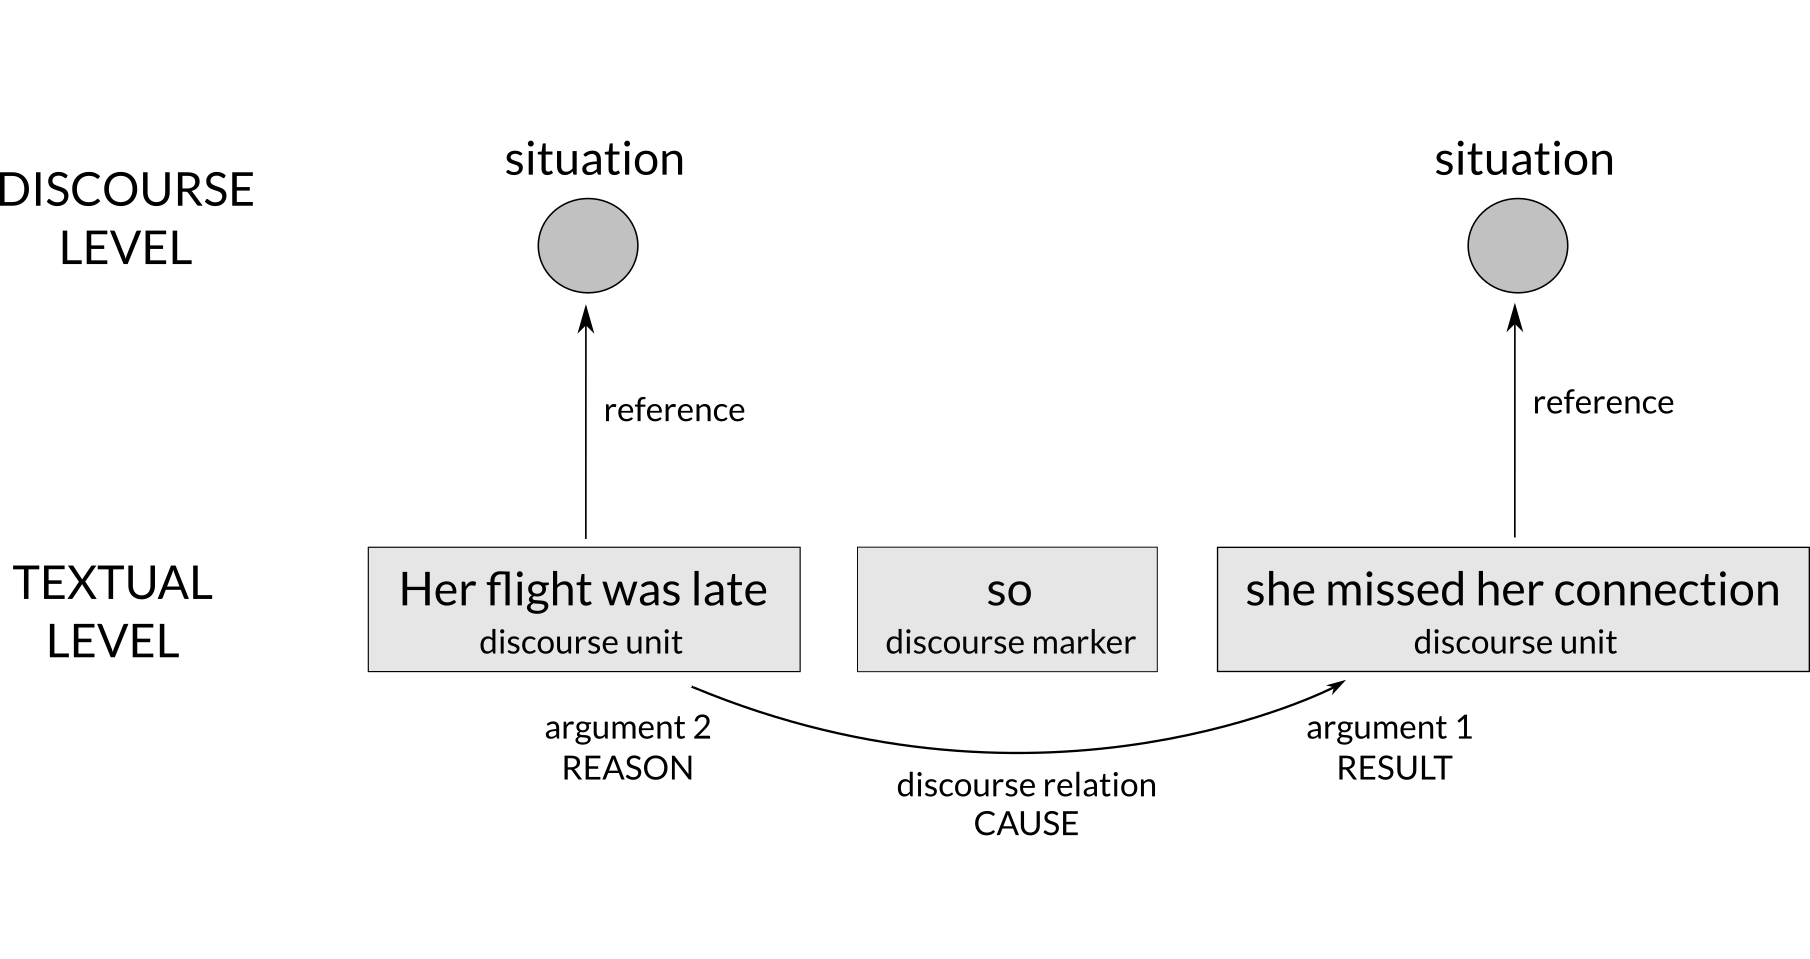
\includegraphics[width=0.9\textwidth]{discourse.png}
\end{center}

%%%%%%%%%%%%%%%%%%%%%%%%%%%%%%%%%%%%%%%%%%%%%%%%%%%%%%%%%%%%%%%%%%%%%%%%%%%%%

\section{The annotation process}

The annotation process includes:

\begin{enumerate}

\item segmentation of the full text into discourse units (see Section~\ref{discourse-units})

\item annotation of the explicit discourse markers (see Section~\ref{discourse-markers})

\item annotation of discourse relations (following the guidelines of the ISO 24617-8 standard, see Section~\ref{discourse-relations}) by:

      \begin{itemize}

      \item indicating the explicit discourse marker signalling the relation, or providing the equivalent implicit relation indicator

      \item specifying the type of relation according to the DR-core schema

      \item indicating the arguments of the relation.

      \end{itemize}

\nonstopmode % this is a hack
\nonstopmode # this is a hack
\end{enumerate}
\errorstopmode
\errorstopmode


%%%%%%%%%%%%%%%%%%%%%%%%%%%%%%%%%%%%%%%%%%%%%%%%%%%%%%%%%%%%%%%%%%%%%%%%%%%%%

\section{Discourse units}
\label{discourse-units}

A discourse unit is a minimal piece of text describing a situation, usually corresponding to a clause.

% % % % % % % % % % % % % % % % % % % % % % % % % % % % % % % % % % % % % % % 

\subsection{Delimitation of discourse units}

Discourse units are determined by the main semantic criterion: they should represent the minimal textual fragments needed to understand a given situation.





% % % % % % % % % % % % % % % % % % % % % % % % % % % % % % % % % % % % % % % 

\subsection{Syntactic constructs representing discourse units}

Below we present examples of syntactic constructs representing discourse units\footnote{Polish examples inspired by \citep[][p.~31--33]{jodlowski1976} and \citep{marcinczuk2016}.}:

\begin{enumerate}

\item construction with the verb in the personal form:

      \begin{itemize}

      \item in the general, self-contained form expressing an event, state, process:

            \begin{ex}
            PL: \textit{Psy \uline{przysiadły} ku ziemi.}
            \end{ex}

            \begin{ex}
            PL: \textit{Mówiła babka, że \uline{był} w~gorącej wodzie kąpany.}
            \end{ex}
            
            \begin{ex}
            PL: \textit{Pamiętnik Deczyńskiego \uline{stał się} źródłem
                pomysłu i~podstawą akcji niniejszej powieści.}
            \end{ex}

      \item in~the modal form completed with an infinitive:

            \begin{ex}
            PL: \textit{Tu i~ówdzie po kątach izby \uline{poczynało się dymić}.}
            \end{ex}

      \end{itemize}

\vspace{5pt}\item construction with the verb in the non-personal form:

      \begin{itemize}

      \item with the impersonal form (PL: \textit{-no}, \textit{-to}):

            \begin{ex}
            PL: \textit{\uline{Skoszono} już 90 procent zbóż}.
            \end{ex}

            \begin{ex}
            PL: \textit{We wsi Wydmuszki Małe \uline{otwarto} sklep samoobsługowy, czyli tak zwany SAM.}
            \end{ex}

      \item with non-reflexive non-personal verb (PL: \textit{trzeba}, \textit{można}):

            \begin{ex}
            PL: \textit{\uline{Trzeba} to sobie umieć powiedzieć.}
            \end{ex}
            \begin{ex}
            PL: \textit{[...] że cierpieniem i patosem od myślenia wykręcić się \uline{można} [...]}
            \end{ex}

      \item With~the non-reflexive momentary verb:

            \begin{ex}
            PL: \textit{(Bierze igłę z nitką), \uline{ciach} mankiet lewy, (ciach prawy, łaty położył niebrzydko).} 
            \end{ex}
            \begin{ex}
            PL: \textit{\uline{Łap} za kota (i lu go na moje łóżko).}
            \end{ex}

      \end{itemize}

\item elliptical construction:

      \begin{itemize}

      \item z~deklinacyjną formą orzecznika:

            \begin{ex}
            PL: \textit{Orłoś jeździeckim \uline{mistrzem} Polski.}
            \end{ex}

      \item z~krótka formą przymiotnika w~roli orzecznika:

            \begin{ex}
            PL: \textit{Znam mego brata, \uline{gotów} na wszystko.}
            \end{ex}
            \begin{ex}
            \textit{\uline{Zdrów} chłop jak rzepa.}
            \end{ex}

      \item z~inną formą orzecznika w~pozycji po podmiocie:

            \begin{ex}
            PL: \textit{(Ale co z poborami?) Kieszeń \uline{sucha}.}
            \end{ex}

            \begin{ex}
            PL: \textit{Siadanie na masce \uline{zabronione}.}
            \end{ex}
            
            \begin{ex}
            PL: \textit{Łazuka \uline{w~modzie}.}
            \end{ex}

      \item z wyrazem \textit{to} w~funkcji łącznika:

            \begin{ex}
            PL: \textit{Samochody \uline{to} nie choinki.}
            \end{ex}

      \item z domysłem predykacji:

            \begin{ex}
            PL: \textit{(— Sam jestem). Żona \uline{na nieszporach.}}
            \end{ex}

      \item z wykładnikiem predykacji realizowanym za pomocą pauzy:

            \begin{ex}
            PL: \textit{Po skonsumowaniu — ziarenka do mnie.}
            \end{ex}

            \begin{ex}
            PL: \textit{Felek już student, Elżunia — panna sklepowa.}
            \end{ex}

            \begin{ex}
            PL: \textit{Telewizor — pedagog.}
            \end{ex}

      \end{itemize}

\item konstrukcja z~rzeczownikiem \textit{żal}, \textit{wstyd},
      \textit{strach}, \textit{pora} itp. stosowanym w~wersji denotatu stanu
      o~funkcji predykatywnej:

            \begin{ex}
            PL: \textit{\uline{Żal} mu bezskuteczności tej walki.}
            \end{ex}

            \begin{ex}
            PL: \textit{(Niech pan tam nawet nie idzie), aż \uline{strach} patrzeć.}
            \end{ex}

\item konstrukcja z~przysłówkiem, zaimkiem przysłownym i~modulantem
      sugerująca możliwość zastosowania czasownika jako ich substratu:

            \begin{ex}
            PL: \textit{\uline{Trudno}, musisz wybierać.}
            \end{ex}

            \begin{ex}
            PL: \textit{(— Tsst, czy już?) — \uline{Już} — ocknęła się Wanda i kiwnęła głową.}
            \end{ex}

\item konstrukcje znominalizowane\footnote{Klasyfikacja zostanie uszczegółowiona na etapie tworzenia instrukcji anotacyjnej.}:

      \begin{itemize}

      \item z~odsłownikiem:

            \begin{ex}
            PL: \textit{Gdyby nie \uline{nadużywanie} napojów alkoholowych, ostatnia sobota mogłaby być zaliczana do spokojnych.} (\textit{Gdyby nie \uline{nadużywano} alkoholu, ...})
            \end{ex}

      \item z~imiesłowem przymiotnikowym:

            \begin{ex}
            PL: \textit{\uline{Nadjeżdżający} pociąg potrącił dwie osoby.} (\textit{Pociąg \uline{nadjechał} i potrącił...})
            \end{ex}

      \item z~rzeczownikiem:

            \begin{ex}
            PL: \textit{\uline{Budowa} domu spędzała mu sen z~powiek.} (\textit{Ktoś \uline{budował} dom i~spędzało mu to sen z~powiek.})\\
            \end{ex}

      \end{itemize}

\nonstopmode % this is a hack
\nonstopmode # this is a hack
\end{enumerate}
\errorstopmode
\errorstopmode


% % % % % % % % % % % % % % % % % % % % % % % % % % % % % % % % % % % % % % % 

\subsection{Annotation decisions}

%   %   %   %   %   %   %   %   %   %   %   %   %   %   %   %   %   %   %   %

\subsubsection{Clause- and sentence-final punctuation}

In general case, final punctuation (sentence-ending dots, clause-ending commas etc.) should be removed from discourse units.

%   %   %   %   %   %   %   %   %   %   %   %   %   %   %   %   %   %   %   %

\section{Discontinuous discourse units}

Discontinuous discourse units are allowed.




%%%%%%%%%%%%%%%%%%%%%%%%%%%%%%%%%%%%%%%%%%%%%%%%%%%%%%%%%%%%%%%%%%%%%%%%%%%%%

\section{Discourse markers}
\label{discourse-markers}

Discourse markers, given explicitly in the~text or implied, link discourse units into relations.


% % % % % % % % % % % % % % % % % % % % % % % % % % % % % % % % % % % % % % % 

\subsection{Annotation decisions}

%   %   %   %   %   %   %   %   %   %   %   %   %   %   %   %   %   %   %   %


\section{Discontinuous discourse markers}

Discontinuous discourse units are allowed and should be marked as a single unit.








%%%%%%%%%%%%%%%%%%%%%%%%%%%%%%%%%%%%%%%%%%%%%%%%%%%%%%%%%%%%%%%%%%%%%%%%%%%%%

\section{Discourse relations}
\label{discourse-relations}

The ISO standard “establishes the representation and annotation of local, »low-level« discourse relations between situations mentioned in discourse, where each relation is annotated independently of other relations in the same discourse” (p.~1). 

The 18~relationships from~the ISO 24617-8:2016 standard a new \textsc{Evaluation} relation from the ISO 24617-2 standard has been added\footnote{According to the intention of the authors of the standard: \textit{The relation ‘Evaluation’ has been added, which has been felt to be missing}‘’ \citep[p.~69]{iso-24617-2}.}.

Discourse relations link a pair of arguments functioning in certain roles, depending on relation name. Unlike other annotation schemes in the~description of relationships asymmetric relations we do not use argument numbers, but their names, which unambiguously indicate the role of the argument. For symmetric relations, we do not give the names of the arguments, treating them equally..


% COMMENT: We should insert here an overview of relations TODO

% % % % % % % % % % % % % % % % % % % % % % % % % % % % % % % % % % % % % % % 

\subsection{Relation inventory}

%   %   %   %   %   %   %   %   %   %   %   %   %   %   %   %   %   %   %   %

\subsubsection{\textsc{Cause}}
%COMMENT: we should insert before USAGE a definition of each relation; then we could have args and examples
%1.Definition + Arg roles 2. Examples: at least 2 examples, at least 1 implicit 3. Diagnostic tests - several examples

%for now: copy ISO relations definitions

%Another idea: inventory of markers (connectives) across languages 

\label{cause}

\renewcommand{\arraystretch}{1.3}
\begin{tabularx}{\textwidth}{|l|L|}
\hline

\textbf{Usage}:           & Arg2 (Reason) is an explanation for Arg1 (Result). \\
\hline

\textbf{Arguments}:       &  \textsc{Reason}: \\
\cline{2-2}
                          &  \textsc{Result}: \\
\hline

\textbf{Markers}:         &  PL: albowiem; bo; bowiem; dlatego; dlatego że; i dlatego; ponieważ; więc; wskutek; w wyniku czego \\
\hline

\end{tabularx}

\begin{enumerate}
\item \textbf{Augsburg relation} Causal\footnote{renamed to avoid confusion between relation "cause" and argument role "reason"} (reason, result)

\nonstopmode % this is a hack
\nonstopmode # this is a hack
\end{enumerate}
\errorstopmode
\errorstopmode


%   %   %   %   %   %   %   %   %   %   %   %   %   %   %   %   %   %   %   %

\subsubsection{\textsc{Condition}}

\renewcommand{\arraystretch}{1.5}
\begin{tabularx}{\textwidth}{|l|L|}
\hline

\textbf{Usage}:           &  Arg2 (Antecedent) is an unrealized situation which, when realized, would lead to
Arg1 (Consequent). \\
\hline

\textbf{Arguments}:       &  \textsc{Antecedent}: \\
\cline{2-2}
                          &  \textsc{Consequent}: \\
\hline

\textbf{Markers}:        &  PL: gdyby…, to…; jak…, to…; jeśli…, to…; …, kiedy…; na wypadek…, …; w przypadku gdy…., to… \\
\hline

\end{tabularx}

\begin{enumerate}
\item \textbf{Augsburg relation} Conditional\noteCC{renamed to avoid confusion with argument role "condition" and for analogy with "causal"} (condition,\noteCC{= antecedent, renamed for disambiguation with terminology from coreference annotation [part of the same schema!]} consequence\noteCC{renamed to avoid confusion with negative condition/consequent})
\nonstopmode # this is a hack
\end{enumerate}
\errorstopmode


%   %   %   %   %   %   %   %   %   %   %   %   %   %   %   %   %   %   %   %

\subsubsection{\textsc{Negative condition}}

\begin{tabularx}{\textwidth}{|l|L|}
\hline

\textbf{Usage}:           &  Arg2 (Negated Antecedent) is an unrealized situation which, when not realized, would lead
to Arg1 (Consequent).\\
\hline

\textbf{Arguments}:       &  \textsc{Negated-antecedent}:  \\
\cline{2-2}
                          &  \textsc{Consequent}: \\
\hline

\textbf{Markers}:        &  PL: albo... albo..., chyba że \\
\hline

\end{tabularx}

\begin{enumerate}[a)]
\item \textbf{Augsburg relation} Negative Condition\noteCC{not renamed, although this is somewhat inconsequential} (neg\_condition,\noteCC{= negated antecedent, renamed for analogy with Condition} neg\_consequence\noteCC{renamed for analogy with Condition})
\nonstopmode # this is a hack
\end{enumerate}
\errorstopmode


%   %   %   %   %   %   %   %   %   %   %   %   %   %   %   %   %   %   %   %

\subsubsection{\textsc{Purpose}}

\begin{tabularx}{\textwidth}{|l|L|}
\hline

\textbf{Usage}:           &  Arg2 (Goal) is the goal or purpose of the situation described by Arg1 (Enablement). \\
\hline

\textbf{Arguments}:       &  \textsc{Enablement}: \\
\cline{2-2}
                          &  \textsc{Goal}: \\
\hline

\textbf{Markers}:         &  PL: aby; poprzez (zrobienie czegoś); więc; w ten sposób; żeby \\
\hline

\end{tabularx}

\begin{enumerate}[a)]
\item \textbf{Augsburg relation} Purpose (goal, enablement)
\nonstopmode # this is a hack
\end{enumerate}
\errorstopmode


%   %   %   %   %   %   %   %   %   %   %   %   %   %   %   %   %   %   %   %

\subsubsection{\textsc{Manner}}

\begin{tabularx}{\textwidth}{|l|L|}
\hline

\textbf{Usage}:           &  Arg2 (Means) specifies how Arg1 (Achievement) comes about or occurs. \\
\hline

\textbf{Arguments}:       &  \textsc{Achievement}: \\
\cline{2-2}
                          &  \textsc{Means}: \\
\hline

\textbf{Markers}:         &  PL: … i tym samym…; … w ten sposób…; … w taki sposób, że…, poprzez… \\
\hline

\end{tabularx}

\begin{enumerate}[a)]
\item \textbf{Augsburg relation} Manner (means, achievement)
\nonstopmode # this is a hack
\end{enumerate}
\errorstopmode


%   %   %   %   %   %   %   %   %   %   %   %   %   %   %   %   %   %   %   %

\subsubsection{\textsc{Concession}}

\begin{tabularx}{\textwidth}{|l|L|}
\hline

\textbf{Usage}:           &  An expected causal relation between Arg1 (Expectation-raiser) and ¬Arg2\\
\hline

\textbf{Arguments}:       &  \textsc{Expectation-raiser}: \\
\cline{2-2}
                          &  \textsc{Expectation-denier}:  \\
\hline

\textbf{Markers}:         &  PL: …, a jednak…; … a mimo wszystko…; chociaż…, to jeszcze nie…; …, choć…; …, natomiast…; …; mimo to…; …, mimo że…; pomimo że…, … \\
\hline

\end{tabularx}

\begin{enumerate}[a)]
\item \textbf{Augsburg relation} Concession (expectation-raiser, contra-expectation)
\nonstopmode # this is a hack
\end{enumerate}
\errorstopmode

        
%   %   %   %   %   %   %   %   %   %   %   %   %   %   %   %   %   %   %   %

\subsubsection{\textsc{Contrast}}

\begin{tabularx}{\textwidth}{|l|L|}
\hline

\textbf{Usage}:           &  One or more differences between Arg1 and Arg2 are highlighted with respect to what each predicates as a whole or to some entities they mention. \\
\hline

\textbf{Arguments}:       &  ... \\
\hline

\textbf{Markers}:        &  PL: ale; podczas gdy; z drugiej strony \\
\hline

\end{tabularx}

\begin{enumerate}[a)]
\item \textbf{Augsburg relation} Contrast
\nonstopmode # this is a hack
\end{enumerate}
\errorstopmode


%   %   %   %   %   %   %   %   %   %   %   %   %   %   %   %   %   %   %   %

\subsubsection{\textsc{Exception}}

\begin{tabularx}{\textwidth}{|l|L|}
\hline

\textbf{Usage}:           &  Arg2 (Exclusion) evokes one or more circumstances in which Arg1 (Regular) does not hold. \\
\hline

\textbf{Arguments}:       &  \textsc{Regular}:  \\
\cline{2-2}
                          &  \textsc{Exclusion}:  \\
\hline

\textbf{Markers}:         &  PL: …, z wyjątkiem tego, że…; …, z zastrzeżeniem, że… \\
\hline

\end{tabularx}

\begin{enumerate}[a)]
\item \textbf{Augsburg relation} Exception (regular, exception)\noteCC{In the Augsburg scheme, we annotate argument roles only for asymmetric relations, as the relation itself can be inferred. These annotations are always anchored at the argument that contains the explicit (or can contain an implicit) discourse marker. The other argument (that a relation points to) then carries the other argument role. As far as we can tell, we would never annotate regular, but always exception.}
\nonstopmode # this is a hack
\end{enumerate}
\errorstopmode


%   %   %   %   %   %   %   %   %   %   %   %   %   %   %   %   %   %   %   %

\subsubsection{\textsc{Similarity}}

\begin{tabularx}{\textwidth}{|l|L|}
\hline

\textbf{Usage}:           &  One or more similarities between Arg1 and Arg2 are highlighted with respect to
what each predicates as a whole or to some entities they mention. \\
\hline

\textbf{Arguments}:       &  ... \\
\hline

\textbf{Markers}:         &  PL: podobnie jak; tak jak \\
\hline

\end{tabularx}

\begin{enumerate}[a)]
\item \textbf{Augsburg relation} Similarity
\nonstopmode # this is a hack
\end{enumerate}
\errorstopmode



%   %   %   %   %   %   %   %   %   %   %   %   %   %   %   %   %   %   %   %

\subsubsection{\textsc{Substitution}}

\begin{tabularx}{\textwidth}{|l|L|}
\hline

\textbf{Usage}:           &  Arg1 (Disfavoured-alternative) and Arg2 (Favoured-alternative) are alternatives, with
Arg2 being the favoured or chosen alternative. \\
\hline

\textbf{Arguments}:       &  \textsc{Disfavoured-alternative}: \\
\cline{2-2}
                          &  \textsc{Favoured-alternative}: \\
\hline

\textbf{Markers}:         &  PL: …, raczej niż…; …, zamiast… \\
\hline

\end{tabularx}


\begin{enumerate}[a)]
\item \textbf{Augsburg relation} Substitution (disfavoured, favoured)\noteCC{renaming is cosmetic, we found `...-alternative' to be redundant, and our annotation involves typing}
\nonstopmode # this is a hack
\end{enumerate}
\errorstopmode

%   %   %   %   %   %   %   %   %   %   %   %   %   %   %   %   %   %   %   %

\subsubsection{\textsc{Conjunction}}

\begin{tabularx}{\textwidth}{|l|L|}
\hline

\textbf{Usage}:           &  Arg1 and Arg2 bear the same relation to some situation evoked in the discourse, explicitly or implicitly. Their conjunction indicates that they both hold with respect to that situation. \\
\hline

\textbf{Arguments}:       &  (symmetric) \\
\hline

\textbf{Markers}:        &  PL: … i …; … i co więcej…; …, a…; …, ale także…; … oraz …; …, zaś… \\
\hline

\end{tabularx}

\begin{enumerate}[a)]
\item \textbf{Augsburg relation} Conjunction
\nonstopmode # this is a hack
\end{enumerate}
\errorstopmode



%   %   %   %   %   %   %   %   %   %   %   %   %   %   %   %   %   %   %   %

\subsubsection{\textsc{Disjunction}}

\begin{tabularx}{\textwidth}{|l|L|}
\hline

\textbf{Usage}:           &  Arg1 and Arg2 bear the same relation to some “situation evoked in the discourse, explicitly or implicitly. Their disjunction indicates that they are alternatives with respect to that situation. The disjunction is non-exclusive so Arg1 and Arg2 may both hold. \\
\hline

\textbf{Arguments}:       &  (symmetric) \\
\hline

\textbf{Markers}:        &  PL: … albo…; albo…, albo… \\
\hline

\end{tabularx}

\begin{enumerate}[a)]
\item \textbf{Augsburg relation} Disjunction
\nonstopmode # this is a hack
\end{enumerate}
\errorstopmode


%   %   %   %   %   %   %   %   %   %   %   %   %   %   %   %   %   %   %   %

\subsubsection{\textsc{Exemplification}}

\begin{tabularx}{\textwidth}{|l|L|}
\hline

\textbf{Usage}:           &  Arg1 (Set) is a set of situations; Arg2 (Instance) is an element of that set. \\
\hline

\textbf{Arguments}:       &  Set:  \\
\cline{2-2}
                          &  Instance:  \\
\hline

\textbf{Markers}:        &  PL: …, czego dowodzi…; …, na przykład…; … w szczególności…; … w tym…  \\
\hline

\end{tabularx}

\begin{enumerate}[a)]
\item \textbf{Augsburg relation} Exemplification (set, instance)
\nonstopmode # this is a hack
\end{enumerate}
\errorstopmode


%   %   %   %   %   %   %   %   %   %   %   %   %   %   %   %   %   %   %   %

\subsubsection{\textsc{Elaboration}}

%\renewcommand{\arraystretch}{1.4}
\begin{tabularx}{\textwidth}{|l|L|}
\hline

\textbf{Usage}:           &  Arg1 (Broad) and Arg2 (Specific) are the same situation, but Arg2 provides more detail. \\
\hline

\textbf{Arguments}:       &  Broad:  \\
\cline{2-2}
                          &  Specific: \\
\hline

\textbf{Markers}:        &  PL: faktycznie; mianowicie; w istocie; w szczególności; ściślej mówiąc \\
\hline

\end{tabularx}

\begin{enumerate}[a)]
\item \textbf{Augsburg relation} Elaboration (broad, specific)\noteCC{as we annotate argument roles, but not the relation, we feel that the labels `broad' and `specific' can be mis-interpreted by annotators, might be renamed to `generalization' and `specification' as in PDTB2. However, definitions remain the same.}
\nonstopmode # this is a hack
\end{enumerate}
\errorstopmode


%   %   %   %   %   %   %   %   %   %   %   %   %   %   %   %   %   %   %   %

\subsubsection{\textsc{Restatement}}

%\renewcommand{\arraystretch}{1.5}
\begin{tabularx}{\textwidth}{|l|L|}
\hline

\textbf{Usage}:           &  Arg1 and Arg2 are the same situation, but viewed from different perspectives. \\
\hline

\textbf{Arguments}:       &  (symmetric) \\
\hline

\textbf{Markers}:        &  PL: …, innymi słowy…; …, inaczej mówiąc… \\
\hline

\end{tabularx}

\begin{enumerate}[a)]
\item \textbf{Augsburg relation} Restatement
\nonstopmode # this is a hack
\end{enumerate}
\errorstopmode



%   %   %   %   %   %   %   %   %   %   %   %   %   %   %   %   %   %   %   %

\subsubsection{\textsc{Synchrony}}

%\setlength{\extrarowheight}{10pt}
\begin{tabularx}{\textwidth}{|l|L|}
\hline

\textbf{Usage}:           &  Some degree of temporal overlap exists between Arg1 (Before) and Arg2 (After). All forms of overlap are included. \\
\hline

\textbf{Arguments}:       &  (symmetric) \\
\hline

\textbf{Markers}:        &  PL: gdy; i jednocześnie; kiedy; podczas gdy \\
\hline

\end{tabularx}

\begin{enumerate}[a)]
\item \textbf{Augsburg relation} Synchrony
\nonstopmode # this is a hack
\end{enumerate}
\errorstopmode



%   %   %   %   %   %   %   %   %   %   %   %   %   %   %   %   %   %   %   %

\subsubsection{\textsc{Asynchrony}}

%\renewcommand{\arraystretch}{1.4}
\begin{tabularx}{\textwidth}{|l|L|}
\hline

\textbf{Usage}:           &  Arg1 temporally precedes Arg2. \\
\hline

\textbf{Arguments}:       &  \textsc{Before}:  \\
\cline{2-2}
                          &  \textsc{After}:  \\
\hline

\textbf{Markers}:        &  PL: a wtedy; aż do momentu, gdy; po tym, jak; zanim \\
\hline

\end{tabularx}

\begin{enumerate}[a)]
\item \textbf{Augsburg relation} Asynchrony (before, after)
\nonstopmode # this is a hack
\end{enumerate}
\errorstopmode


%   %   %   %   %   %   %   %   %   %   %   %   %   %   %   %   %   %   %   %

\subsubsection{\textsc{Expansion}}

%\renewcommand{\arraystretch}{1.5}
\begin{tabularx}{\textwidth}{|l|L|}
\hline

\textbf{Usage}:           &  Arg2 (Expander) is a situation involving some entity/entities in Arg1 (Narrative), expanding the narrative of which Arg1 is a part, or expanding on the setting relevant for interpreting Arg1. The Arg1 and Arg2 situations are distinct. \\
\hline

\textbf{Arguments}:       &  \textsc{Narrative}: \\
\cline{2-2}
                          &  \textsc{Expander}: \\
\hline

\textbf{Markers}:        &  PL: i (or no marker) \\
\hline

\end{tabularx}

\paragraph{Notes} 

\begin{itemize}
\item Typically, these relations are implicit and do not allow insertion of a connective to
express the relation. In English, “and” can be used when Expansion carries the narrative
forward. (p.20)
\item \textbf{Augsburg relation} \textbf{RENAMED TO/MERGED WITH EntRel}: We use the PDTB2-top level categories for classifying discourse relations in the guidelines (not directly for annotation), because our manual is based on a synthesis between ISO definitions and PDTB2 (not PDTB3) documentation. When trying to narrow down the definition to sufficient and necessary conditions, we felt that the "involving some entity part" would be necessary, whereas the disjunction ("expanding ..., or expanding ...") would be sufficient. As a result, we identified that with the PDTB2 relation EntRel, plus adding the constraint that it must be a(n Expansion) relation for cases where no other relation applies. (This could be revoked.)
\nonstopmode # this is a hack
\end{enumerate}
\errorstopmode


\vfill\clearpage


%   %   %   %   %   %   %   %   %   %   %   %   %   %   %   %   %   %   %   %

\subsubsection{\textsc{Evaluation}}

\renewcommand{\arraystretch}{1.5}
\begin{tabularx}{\textwidth}{|l|L|}
\hline

\textbf{Usage}:           &  ... \\
\hline

\textbf{Arguments}:       &  \textsc{Situation}: \\
\cline{2-2}
                          &  \textsc{Judgement}: \\
\hline

\textbf{Markers}:         &  PL: i (or no marker) \\
\hline

\end{tabularx}

\paragraph{Notes}

\begin{enumerate}[a)]
\item \emph{CC, Nov 2024} missing in ISO
\nonstopmode # this is a hack
\end{enumerate}
\errorstopmode

%   %   %   %   %   %   %   %   %   %   %   %   %   %   %   %   %   %   %   %

\subsubsection{\textsc{Functional dependence}}

\renewcommand{\arraystretch}{1.4}
\begin{tabularx}{\textwidth}{|l|L|}
\hline

\textbf{Usage}:           &  (defined via argument roles) \\
\hline

\textbf{Arguments}:       &  \textsc{Antecedent-act}: Arg1 (Antecedent-act) is the dialogue act that Arg2 responds to.\\
\cline{2-2}
                          &  \textsc{Dependent-act}: Arg2 (Dependent-act) is a dialogue act with a responsive communicative function \\
\hline

\end{tabularx}

\paragraph{Notes}

\begin{enumerate}[a)]
\item Due to its responsive character, the determination of the semantic content of Arg2 in general requires determination of the semantic content of Arg1. (ISO, p.20)
\item Responsive dialogue acts, defined in ISO 24617-2, are: Agreement, Disagreement, Answer, Confirm, Disconfirm, Correction, Accept Request, Decline Request, Address Request, Accept Offer, Decline Offer, Address Offer, Accept Suggest, Decline Suggest, Address Suggest, Return Greeting, Return Self-Introduction, Accept Apology, Accept Thanking, and Return Goodbye. (ISO, p.20)
\item This relation cannot be expressed by a discourse connective. (ISO, p.20)
\item \emph{Nov 2024, Augsburg meeting}: Do not annotate, for the moment.
\nonstopmode # this is a hack
\end{enumerate}
\errorstopmode


%   %   %   %   %   %   %   %   %   %   %   %   %   %   %   %   %   %   %   %

\subsubsection{\textsc{Feedback dependence}}

\begin{tabularx}{\textwidth}{|l|L|}
\hline

\textbf{Usage}:           &  Arg2 is a dialogue act with a feedback function that provides or elicits information
about the understanding or evaluation by one of the dialogue participants of Arg1. \\
\hline

\textbf{Arguments}:       &  \textsc{Feedback-scope}: \\
\cline{2-2}
                          &  \textsc{Feedback-act}: \\
\hline

\end{tabularx}

\paragraph{Notes}

\begin{enumerate}[a)]
\item The semantic content of Arg2 is mostly provided by Arg1. (ISO, p.21)
\item The ISO standard for dialogue act annotation (ISO 24617-2) defines five feedback functions:
Auto-Positive and Auto-Negative, providing positive and negative feedback information,
respectively, about the speaker’s processing of something that was said by another speaker;
Allo-Positive and Allo-Negative, similarly about the addressee’s processing of something
that the speaker has said; and Feedback Elicitation, eliciting feedback about the addressee’s
processing of something that the speaker has said. (ISO, p. 21)
\item 
This relation cannot be expressed by a discourse connective, but is often expressed in English
by “OK”, “right”, “pardon?” and in similar ways in other languages. (ISO, p. 21)
\item \emph{Nov 2024, Augsburg meeting}: Do not annotate, for the moment.
\nonstopmode # this is a hack
\end{enumerate}
\errorstopmode

% % % % % % % % % % % % % % % % % % % % % % % % % % % % % % % % % % % % % % % 

\subsection{Annotation Problems}

In the process of annotating discourse relations, several challenges have been identified. This section discusses these problems and proposes resolutions to ensure consistency and accuracy in the annotation.

\subsubsection{Argument Identification and Scope}

\subsubsection{Problem 1: Defining Argument Scope}

One of the primary challenges is determining the scope of arguments and the spans within the text that constitute these arguments. Specifically, deciding which elements in a sentence or phrase should be included in the argument span can be problematic.

\textbf{Proposed Resolution:} Utilize syntactic criteria, such as syntactic parsers, to define argument boundaries. Develop diagnostic tests or questions to assist in identifying the scope. For instance, in the case of a \textsc{Cause} relation, one might ask:

\begin{itemize}
    \item What is the reason for \textit{Arg\textsubscript{x}}?
    \item What is the result for \textit{Arg\textsubscript{y}}?
\end{itemize}

\textbf{Example:}

\begin{quote}
They ate provisions and gnawed at lines of rope, \textbf{so} cats had long since become essential sailing companions.
\end{quote}

Applying the diagnostic questions:

\begin{itemize}
    \item \textit{What is the reason for cats becoming essential sailing companions?} \\
    They ate provisions and gnawed at lines of rope.
    \item \textit{What is the result of them eating provisions and gnawing at lines of rope?} \\
    Cats had long since become essential sailing companions.
\end{itemize}

Similarly, for other relations, appropriate questions can be formulated:

\begin{itemize}
    \item \textsc{Expansion}: What else is said about \textit{Arg\textsubscript{x}}? What is the topic of \textit{Arg\textsubscript{y}}?
    \item \textsc{Asynchrony}: What happened before \textit{Arg\textsubscript{x}}? What happened after \textit{Arg\textsubscript{y}}?
    \item \textsc{Elaboration}: What situation is part of \textit{Arg\textsubscript{x}}?
\end{itemize}

\subsubsection{Problem 2: Constituting an Argument}

Determining what constitutes a single argument poses a challenge, particularly when considering whether events represented by nouns can serve as arguments.

\textbf{Proposed Resolution:} An argument of a discourse relation can be a clause, nominal eventuality, sentence, or a set of sentences. Thus, events represented by nouns can be considered as arguments if they denote situations.

\textbf{Example:}

\begin{quote}
The rain caused \textbf{damage to the building}.
\end{quote}

In this example, \textit{damage to the building} is a nominal eventuality that serves as an argument.

\subsubsection{Problem 3: Inclusion of Connectives in Arguments}

Another issue is whether the connective (discourse marker) should be considered part of the argument span.

\textbf{Proposed Resolution:} Include the connective as part of the argument. This approach ensures that the connective's role in signaling the relation is preserved within the argument structure.

\subsection{Discourse Relation Assignment}

\subsubsection{Problem 4: Overlapping Relations}

Instances may arise where an example can be interpreted according to the definitions of two distinct discourse relations, leading to ambiguity.

\textbf{Proposed Resolution:} If both relations apply equally, annotate both. When one is more prevalent than the other (%how to decide?), annotate only the most salient one or rank the options based on their prominence.

\textbf{Examples:}

\begin{itemize}
    \item \textbf{Cause:} Having eaten the soup, John was allowed to leave the table.
    \item \textbf{Asynchrony:} Having eaten the soup, John left the table.
    \item \textbf{Asynchrony and Conjunction:} They sold their core power tools business and reinvested those proceeds in a water business.
\end{itemize}

\subsubsection{Problem 5: Imprecise Definitions}

Some discourse relations, such as \textsc{Expansion} and \textsc{Elaboration}, may have less clearly defined boundaries, leading to confusion during annotation.

\textbf{Proposed Resolution:} Refine the definitions by incorporating distinguishing features of those discourse relations, such as temporal characteristics (e.g., temporal inclusion for \textsc{Elaboration}). Develop a decision tree or prioritization guidelines to aid in assigning relations consistently.

\subsubsection{Problem 7: Directionality of Arguments}

There is uncertainty regarding whether to assign argument roles according to the linear order of discourse or regardless of order, as specified in the ISO standard.

\textbf{Proposed Resolution:} Although the ISO standard assigns argument roles regardless of linear order, it may be more intuitive to follow the linear order of discourse. Therefore, assign roles based on the sequence in which arguments appear in the text.

\subsection{Connectives}

\subsubsection{Problem 8: Definition of Connectives}

Clarifying what constitutes a connective and determining which markers should be considered in the annotation process is essential.

\textbf{Proposed Resolution:} Adopt a similar approach to the Penn Discourse Treebank (PDTB) by considering conjunctions, adverbials, and prepositional phrase adverbs as connectives. This provides a clear guideline for identifying discourse markers.

\subsection{Dialogue Acts}

\subsubsection{Problem 9: Dialogue Relations in Monologues}

Challenges arise when dialogue relations, such as \textsc{Functional Dependence} or \textsc{Feedback Dependence}, appear within monologues.

\textbf{Proposed Resolution:} Utilize ISO 24617-2 (Part~2) on Dialogue Acts to handle dialogue-specific discourse relations (so that dialogue elements are appropriately annotated within monologic texts).

\vspace{12pt}




\subsection{Annotation decisions}

%   %   %   %   %   %   %   %   %   %   %   %   %   %   %   %   %   %   %   %

\subsubsection{Multiple relations}

Multiple relations are allowed:

\begin{quote}
    “the specification provides for representing multiple relations inferred between two given situations, both when the relations are realized explicitly as well as implicitly” (p. 5)
\end{quote}


%   %   %   %   %   %   %   %   %   %   %   %   %   %   %   %   %   %   %   %

\subsubsection{Custom names of discourse relations}

Custom names of discourse relations are not allowed.


%   %   %   %   %   %   %   %   %   %   %   %   %   %   %   %   %   %   %   %

\subsubsection{Hierarchy of discourse relations}

Discourse relations do not form a hierarchy:

\begin{quote}
    “the solution adopted in the DR-core specification is to use a »flat« set of core relations that can be used in an annotation scheme as just that, or mapped to the appropriate type within a particular hierarchical scheme adopted” (p. 5)
\end{quote}

%   %   %   %   %   %   %   %   %   %   %   %   %   %   %   %   %   %   %   %

\subsubsection{(A)symmetry of relations}

\begin{quote}
    “asymmetry is represented by specifying the argument roles in the definition of each relation. (...) For example (...) the text span named Arg2 always provides the reason in the Cause relation, irrespective of linear order or syntax, and Arg1 always constitutes the result. In symmetric relations, on the other hand, where both arguments play the same semantic role, arguments are named Arg1 and Arg2 following their linear order in the text.” (p. 6)
\end{quote}

%   %   %   %   %   %   %   %   %   %   %   %   %   %   %   %   %   %   %   %

\subsubsection{Discourse segmentation}

“what counts as a DRel argument is constrained by its semantic status rather than its syntactic form. In particular, a DRel argument must denote a situation (...) of the following types: event, state, fact, proposition, or dialogue act” (p. 7)

%   %   %   %   %   %   %   %   %   %   %   %   %   %   %   %   %   %   %   %

\subsubsection{Arity of arguments}

\begin{quote}
    “a discourse relation is restricted to two and only two arguments” (p. 7)
\end{quote}

%   %   %   %   %   %   %   %   %   %   %   %   %   %   %   %   %   %   %   %

\subsubsection{syntactic form, extent, and (non-)adjacency of argument realizations}

\begin{quote}
“what counts as a DRel argument is constrained by its semantic status rather than its syntactic form”\\
“the DR-core specification remains neutral on the issues of the extent and adjacency of argument spans and does not specify any constraints” (p. 7)
\end{quote}

\subsubsection{Triggers of discourse relations}

\begin{quote}
“it is considered important to explicitly mark expressions seen as the textual triggers of DRels, since these are valuable clues for inducing models for discourse processing. However, the scheme is flexible about the inference sites for implicit DRels, that is, whether implicit DRels are allowed only between adjacent discourse units or between non-adjacent units as well.” \\
“insertion of connectives to express inferred DRels is allowed but not required” (p. 8)
\end{quote}

\subsubsection{Attribution as a discourse relation}

\begin{quote}
“The annotation of attribution is recommended as a separate layer, to be undertaken according to a separate annotation scheme. Interactions of attributions with discourse relations can then be utilized by merging the two layers of annotation.” (p. 9)
\end{quote}

\subsubsection{Representation of entity-based relations}

\begin{quote}
“the current specification provides for only a single relation to capture these entity-based relations, called »Expansion«. In the future, the second part of the project, of which DR-core forms the first part, should clarify this relation and capture more fine-grained distinctions.” (p. 10)
\end{quote}

\subsubsection{Representation of non-existence of a discourse relation}

\begin{quote}
“to accommodate annotation frameworks that impose strict adjacency constraints on the marking of relations, the label »NoRelation«” can be utilized when two adjacent segments are not related by any discourse relation” (p. 11)
\end{quote}

\subsubsection{Inventory of discourse relations (labels, definitions, argument roles)}

\begin{quote}
“the DR-core set of core discourse relations is based on the establishment of semantic equivalences with five well-known semantic taxonomies for discourse relations: PDTB, HTDC, RST, SDRT and CCR. (...) The level of granularity is motivated by the consideration that the chosen relations encapsulate the minimal description that has been more or less successfully implemented in various annotation efforts to date. This set is by no means fixed and can be augmented in three ways: (1) with more fine-grained refinements of the core relations; (2) with less fine-grained abstractions of the core relations; and (3) with equally fine-grained relations that may supplement the set of core relations.” (pp. 12–13)
\end{quote}


In our annotation we make the following general assumptions:

\begin{itemize}

\item Pragmatic issues (representations of beliefs or acts of
dialogical acts) are represented outside the layer of discursive relations,

\item the list of relations should remain flat; eventually it may be
expanded, but we assume that most uncertainties should be able to be
resolved at the super-annotation stage by selecting relations from~the set of
DR-core or by adding a designation binding the relation to~another layer of the
metatextual layer; we assume that we adopt for~this purpose the method of annotation from~PDC
0.5, i.e. marking uncertain relations with additional tags.

\end{itemize}


\begin{enumerate}[a)]
\item \textbf{on Augsburg} I added a few notes on correspondences with our schema. These are not meant to stay, but serve as anchors to check wether definitions and examples have been compared, already.

\item \textbf{Augsburg relations} The Augsburg schema follows ISO definitions, but using the (more exhaustive) PDTB documentation, notes and examples to flesh them out. Also, we provide an exhaustive annotation of intersentential relations in the sense that we annotate every sentence (as predicted by automated parser) with exactly one relations. To achieve this, we had to add 

      \begin{itemize}
      \item \textsc{Hypophora} (from PDTB3) for rhetorical questions
      \item \textsc{Attribution} (similar to RST), but only for a statement separated from its attribution. So far, all examples we know of are incorrectly separated by parser errors or weird paragraph breaks in the source.
      \item \textsc{EntRel} (from PDTB3, but identified with ISO \textsc{Expansion}). Other than PDTB, we consider EntRel to be a part of the top-level category Expansion.
      \end{itemize}

Also, we did not abandon functional-dependence and feedback dependence, annotated by their respective sub-types. (But so far, they did not occur in our data.)

\item \textbf{Augsburg arguments} The Augsburg schema is focusing on intersentential linking, i.e., our arguments are normally (the main eventualities of) sentences, not spans. Our annotation is inspired by the UD treatment of relative clauses: 
      
      \begin{itemize}
      \item discourse relations exist between a sentence (`anchor', corresponds to UD dependent) and a context sentence from the local context (`target', corresponds to UD head)
      \item optionally, an anchor can carry a discourse marker (hence the name, corresponds to UD \texttt{mark})
      \item for symmetric relations, we annotate the first element as target, the second as anchor
      \item for asymmetric relation, we annotate the argument role of the anchor element (relation is inferred)
      \item discourse markers are included in the anchor
      \end{itemize}

This is a temporary informative note relevant for comparing definitions. To be omitted from the guideline document.

\nonstopmode # this is a hack
\end{enumerate}
\errorstopmode


%%%%%%%%%%%%%%%%%%%%%%%%%%%%%%%%%%%%%%%%%%%%%%%%%%%%%%%%%%%%%%%%%%%%%%%%%%%%%

\section*{Acknowledgements}

This research was funded by National Science Centre, Poland, grant 2023/50/A/HS2/00559. 

\bibliography{iso}
\bibliographystyle{udisc}

\end{document}
